\section{Скользящие режимы}
\label{sec:sliding}

\subsection{Системы с переменной структурой}
\lecture{L6}{1--6}

У системы с переменной структурой правая часть меняется при переходе через
некоторую границу в пространстве состояний. Разные области имеют разные
векторные поля. Граница называется поверхностью переключения. В естественных
системах переключение обусловлено физикой, например сухим трением.
В искусственных системах его задаёт регулятор. Лекция различает создание
движения вдоль устойчивых фазовых траекторий и собственно скользящий режим,
при котором переключение создаёт движение, не совпадающее с обычной
траекторией каждого из двух отдельных полей.

Главная идея управления: сначала притянуть состояние к выбранной поверхности,
затем обеспечить устойчивую динамику вдоль неё. Эти два требования нужно
проверять по отдельности. Удобная поверхность без притяжения к ней не решает
задачу; притягивающая поверхность с неустойчивым движением вдоль неё тоже
не обеспечивает стабилизацию.

\subsubsection{Пример сухого трения}

В лекции рассматривается пружинная система $\ddot x+\omega_0^2x=0$
с силой трения постоянного модуля $\omega_0^2\varepsilon$, направленной
против скорости. При ненулевой скорости физически согласованная запись имеет
вид
\[
 \ddot x=-\omega_0^2x-\omega_0^2\varepsilon\sgn\dot x
 =\begin{cases}
  -\omega_0^2(x-\varepsilon),&\dot x<0,\\
  -\omega_0^2(x+\varepsilon),&\dot x>0.
 \end{cases}
\]
Если скорость уже равна нулю, статическое трение может удерживать пружину
при $|\omega_0^2x|\le\omega_0^2\varepsilon$, то есть $|x|\le\varepsilon$.
Поэтому получается целый интервал покоя, а не единственное равновесие $x=0$.

На фазовой плоскости $y=\dot x$ участки движения являются дугами эллипсов
гармонического осциллятора, сдвинутых относительно начала координат на
$\pm\varepsilon$. После смены знака скорости меняется центр соответствующей
дуги. Механическая энергия
\[
 E=\frac{y^2+\omega_0^2x^2}{2},\qquad
 \dot E=-\omega_0^2\varepsilon|y|\le0
\]
убывает. Траектория может закончиться в любой допустимой точке покоя.

\addition Условие $|x|>\varepsilon$ относится к возможности начать движение
из состояния покоя. При уже ненулевой скорости система может двигаться и
внутри полосы $|x|\le\varepsilon$. В записи по случаям эти ситуации нельзя
смешивать. Убывание энергии в данном примере не доказывает притяжение
именно к $x=0$, поскольку множество равновесий не одноточечное.

\subsubsection{Релейное переключение двух линейных полей}

Во втором примере
\[
 \ddot x=\omega_0^2xu,\qquad y=\dot x,\qquad
 u=-\sgn\bigl[(y+\omega_0x)x\bigr].
\]
Здесь $u$ принимает значения $\pm1$. При $u=1$ имеется седло с прямыми
$y=\pm\omega_0x$; прямая $y=-\omega_0x$ является его устойчивой асимптотой.
При $u=-1$ получается центр: $\ddot x=-\omega_0^2x$.
Линиями переключения выбраны $x=0$ и $y+\omega_0x=0$.
Такое управление объединяет участки траекторий центра и седла, направляя
движение к устойчивой асимптоте. На ней при $u=1$ выполняется
$\dot x=-\omega_0x$, следовательно, $x(t)\to0$.
Рисунок лекции показывает именно сборку нужного фазового движения из
траекторий двух структур. Здесь входной коэффициент $\omega_0^2x$ меняет
знак и обращается в нуль, поэтому последующую теорему для $g(x)\ge g_0>0$
к этому примеру напрямую применять нельзя.

\subsubsection{Релейное управление двойным интегратором}

Для $\ddot x=u$ в лекции выбраны
\[
 y=\dot x,\qquad \sigma=x+\alpha y,\qquad
 u=-\sgn\sigma,\qquad \alpha>0.
\]
На $\sigma=0$ скорость связана с положением: $\dot x=y=-x/\alpha$.
Это устойчивая динамика по поверхности. При постоянном $u=\pm1$ обычные
фазовые траектории удовлетворяют $y^2-2ux=\text{const}$ и являются параболами;
переключение соединяет их с движением по наклонной прямой.

\addition Проверка притяжения делается через
$\dot\sigma=y+\alpha u$. Со стороны $\sigma>0$ требуется
$y-\alpha<0$, со стороны $\sigma<0$ --- $y+\alpha>0$.
Таким образом, строгий режим притяжения обеими структурами имеет место
на участке $|y|<\alpha$. Само уравнение прямой не является доказательством
существования скольжения во всех её точках.

\subsection{Выбор поверхности и достаточного усиления}
\lecture{L6}{7--9}

Общий объект лекции имеет вид
\begin{equation}
 \dot x_1=x_2,\qquad
 \dot x_2=h(x)+g(x)u,\qquad g(x)\ge g_0>0.
 \label{eq:sm-general}
\end{equation}
Положительный нижний предел $g_0$ означает известный знак эффективности
управления и отсутствие вырождения входного канала. Для выбранного
$a_1>0$ вводится
\[
 s=a_1x_1+x_2.
\]
На поверхности $s=0$ имеем $\dot x_1=-a_1x_1$ и $x_2=-a_1x_1$.
Число $a_1$ задаёт скорость затухания движения вдоль поверхности.
Производная функции переключения:
\[
 \dot s=a_1x_2+h(x)+g(x)u.
\]
Неизвестные слагаемые нужно оценить, а не подставить их истинные значения
в регулятор. Пусть известна неотрицательная функция $\varrho$ такая, что
\begin{equation}
 \left|\frac{a_1x_2+h(x)}{g(x)}\right|\le\varrho(x).
 \label{eq:sm-rho}
\end{equation}
Символ $\varrho$ здесь означает оценку неопределённости. Это другая величина,
чем относительная степень $\rho$ из темы линеаризации.

Выбирают положительный запас $\beta_0$ и закон
\begin{equation}
 \beta(x)\ge\varrho(x)+\beta_0,\qquad
 u=-\beta(x)\sgn s,\qquad \beta_0>0.
 \label{eq:sm-law}
\end{equation}
При $s>0$ управление отрицательно, при $s<0$ положительно. С помощью
$V=s^2/2$ обе области анализируются одной цепочкой:
\begin{align*}
 \dot V&=s[a_1x_2+h(x)]-g(x)\beta(x)|s|\\
 &\le g(x)|s|\varrho(x)-g(x)\beta(x)|s|\\
 &\le-g(x)\beta_0|s|\le-g_0\beta_0|s|
 =-g_0\beta_0\sqrt{2V}.
\end{align*}
Для $s\ne0$ эквивалентно $\frac{d}{dt}|s|\le-g_0\beta_0$.
Интегрирование даёт конечное время достижения
\begin{equation}
 t_*\le\frac{|s(0)|}{g_0\beta_0}.
 \label{eq:sm-time}
\end{equation}
Это время достижения \emph{поверхности}, а не начала координат.
После достижения координаты затухают экспоненциально и обычно становятся
точно нулевыми лишь в пределе $t\to\infty$.

\addition Для глобального вывода нужно также исключить уход решения на
бесконечность до $t_*$. В~\eqref{eq:sm-general} это следует из ограниченности
$s$ и уравнения $\dot x_1=-a_1x_1+s$: сначала ограничен $x_1$, затем
$x_2=s-a_1x_1$. При наличии дополнительных внутренних координат их
ограниченность придётся доказывать отдельно, как при нуль-динамике.

\subsection{Что означает движение на поверхности}
\addition В обычном программном определении $\sgn0=0$. Если просто подставить
его в объект, в точке $s=0$ обычно получится $\dot s\ne0$. Это не модель
идеального скольжения. Разрывный закон рассматривается в смысле Филиппова:
на поверхности допустимы усреднённые значения управления из
$[-\beta(x),\beta(x)]$.

Управление, поддерживающее $\dot s=0$, называется эквивалентным:
\[
 u_{eq}=-\frac{a_1x_2+h(x)}{g(x)}.
\]
Условие~\eqref{eq:sm-rho} и запас усиления обеспечивают
$|u_{eq}|\le\varrho<\beta$. Поэтому необходимая средняя компенсация
действительно лежит между уровнями реле.

При синтезе реального закона истинное $h$ может быть неизвестно;
в регулятор входит его гарантированная оценка $\varrho$.
При моделировании объекта истинные параметры задаются, поэтому
$u_{eq}$ можно вычислить для изображения идеального скользящего участка.
Это не означает, что робастный регулятор должен знать эти параметры.

\subsection{Частые переключения и номинальная компенсация}
\lecture{L6}{10--11}

В идеальной модели переключение происходит без задержки. В реальном контуре
есть дискретность измерения, задержка вычислений и динамика исполнительного
устройства. Пока управление переключается, состояние пересекает поверхность,
поэтому возникают частые колебания вокруг неё --- chattering.
Высокочастотное переключение может нагружать привод и возбуждать
неучтённую динамику. Один путь из лекции --- уменьшить требуемую разрывную
часть с помощью номинальной компенсации.

Пусть доступны $\hat h(x)$, $\hat g(x)\ne0$. Выбирается
\begin{equation}
 u=-\frac{a_1x_2+\hat h(x)}{\hat g(x)}+v.
 \label{eq:sm-nominal}
\end{equation}
После подстановки
\[
 \dot s=\delta(x)+g(x)v,
\]
\[
 \delta(x)=a_1\left(1-\frac{g(x)}{\hat g(x)}\right)x_2
       +h(x)-\frac{g(x)}{\hat g(x)}\hat h(x).
\]
Если $|\delta(x)/g(x)|\le\varrho(x)$, достаточно выбрать
$v=-\beta(x)\sgn s$, $\beta\ge\varrho+\beta_0$.
Оценивается теперь только ошибка номинальной модели, а не вся правая часть.
При точной модели $\delta=0$.

\textbf{Уточнение записи лекции.} В формуле компенсации нужен минус перед
дробью: именно он приводит к показанному в лекции выражению для $\delta$.
Это легко проверить прямой подстановкой в $\dot s$.
При достаточно точной номинальной модели компенсация может уменьшить
амплитуду релейной части,
но не делает закон полностью непрерывным.

\subsection{Непрерывный регулятор с насыщением}
\lecture{L6}{12--14}

Второй путь из лекции --- заменить знак непрерывной функцией
\[
 \sat y=\begin{cases}y,&|y|\le1,\\\sgn y,&|y|>1,\end{cases}
 \qquad
 u=-\beta(x)\sat\left(\frac{s}{\varepsilon}\right),\quad\varepsilon>0.
\]
За пределами полосы $|s|\le\varepsilon$ этот закон совпадает с реле.
Поэтому при прежних предпосылках полоса достигается за
\[
 t_\varepsilon\le
 \frac{\max\{|s(0)|-\varepsilon,0\}}{g_0\beta_0}
\]
и остаётся инвариантной: на её границах поле направлено внутрь.
В полосе управление равно $-\beta s/\varepsilon$ и непрерывно проходит
через нуль. Коэффициент $\beta/\varepsilon$ определяет крутизну.

\addition При произвольной ненулевой неопределённости гарантируется малая
окрестность, а не автоматически точная асимптотическая стабилизация.
Действительно, внутри полосы
\[
 \dot V\le g(x)|s|\varrho(x)-\frac{g(x)\beta(x)}{\varepsilon}s^2,
\]
и слагаемое порядка $|s|$ может превосходить отрицательное квадратичное
слагаемое при малом $s$. Для системы~\eqref{eq:sm-general} из
$\dot x_1=-a_1x_1+s$ получается
\[
 \limsup_{t\to\infty}|x_1(t)|\le\frac{\varepsilon}{a_1},\qquad
 \limsup_{t\to\infty}|x_2(t)|\le2\varepsilon.
\]
При уменьшении $\varepsilon$ улучшается гарантируемая точность, но растут
крутизна управления и требования к скорости привода и численному шагу.
Непрерывность закона по состоянию и малость ошибки являются разными свойствами.

Слайды 13--14 показывают применения скользящего управления к шару на колесе
и шару на сфере. Они иллюстрируют выбор поверхности для нелинейного объекта
и подавление неопределённости переключающей частью; отдельной новой формулы
синтеза на этих слайдах нет.

\subsection{Работа 5 Первая система и выбор поверхности}
\label{subsec:sm-lab1}
\addition Рассмотрим
\[
 \dot x_1=x_2+\sin x_1,\qquad
 \dot x_2=\theta_1x_1^2+(2+\theta_2)u,\qquad |\theta_1|,|\theta_2|\le1.
\]
Линейную поверхность нельзя выбирать вслепую: первое уравнение содержит
дополнительное $\sin x_1$. Чтобы точно получить нужную динамику на
поверхности, выберем
\[
 s=x_1+x_2+\sin x_1.
\]
Тогда $\dot x_1=-x_1+s$, а при $s=0$ --- $\dot x_1=-x_1$.
Внешняя переменная $x_2+\sin x_1$ измерима через состояние, неизвестных
параметров в определении $s$ нет. Точное дифференцирование даёт
\[
 \dot s=(1+\cos x_1)(x_2+\sin x_1)+\theta_1x_1^2+(2+\theta_2)u.
\]
Поскольку $2+\theta_2\in[1,3]$, подходят
\begin{equation}
 \varrho(x)=|(1+\cos x_1)(x_2+\sin x_1)|+x_1^2,\qquad
 \beta(x)=\varrho(x)+1.
 \label{eq:sm-lab1-gain}
\end{equation}
Здесь $x_1^2$ оценивает неизвестное $\theta_1x_1^2$, а деление на
неизвестный входной коэффициент заменено его нижней границей $1$.
Это несколько консервативная, но реализуемая оценка.

\subsubsection{Разрывный закон и устойчивость}

Для $u=-\beta\sgn s$ получаем
\[
 V=\frac{s^2}{2},\qquad
 \dot V\le-(2+\theta_2)|s|\le-|s|,\qquad t_*\le|s(0)|.
\]
До достижения поверхности $s$ ограничен, а $\dot x_1=-x_1+s$ обеспечивает
ограниченность $x_1$. Далее $x_2=s-x_1-\sin x_1$ тоже ограничен.
На поверхности $x_1(t)=x_1(t_*)e^{-(t-t_*)}$ и
$x_2=-x_1-\sin x_1\to0$. Малые начальные состояния дают малые $s(0)$
и малые состояния до достижения, поэтому имеется и устойчивость, и
глобальное притяжение: начало глобально асимптотически устойчиво.

Для моделирования идеального скольжения используется
\[
 u_{eq}=\frac{(1+\cos x_1)x_1-\theta_1x_1^2}{2+\theta_2}.
\]
Знак получается из условия $\dot s=0$ после подстановки
$x_2+\sin x_1=-x_1$.

\subsubsection{Почему непрерывный закон здесь тоже приводит точно к нулю}

Возьмём ту же $\beta$ и
\[
 u=-\beta\sat(s/\varepsilon),\qquad 0<\varepsilon\le\frac14.
\]
Сначала достигается инвариантная полоса $|s|\le\varepsilon$ за время
не более $\max\{|s(0)|-\varepsilon,0\}$. В отличие от общего случая,
неопределённые слагаемые здесь исчезают в нуле. Это позволяет доказать
более сильный результат с помощью полной функции
$V_c=(x_1^2+s^2)/2$.
Внутри полосы имеем
\begin{align*}
 \dot V_c={}&-x_1^2-\cos x_1\,x_1s+(1+\cos x_1)s^2
       +\theta_1x_1^2s-\frac{(2+\theta_2)\beta}{\varepsilon}s^2.
\end{align*}
Оцениваем смешанные слагаемые неравенством Юнга:
\[
 |x_1s|+x_1^2|s|
 =|x_1|(1+|x_1|)|s|
 \le\frac{x_1^2}{2}+\frac{(1+|x_1|)^2s^2}{2}
 \le\frac{x_1^2}{2}+(1+x_1^2)s^2.
\]
Учитывая $1+\cos x_1\le2$, $2+\theta_2\ge1$ и
$\beta\ge1+x_1^2$, получаем
\[
 \dot V_c\le-\frac{x_1^2}{2}
 +\left(3+x_1^2-\frac{\beta}{\varepsilon}\right)s^2
 \le-\frac{x_1^2}{2}-(1+3x_1^2)s^2\le-V_c.
\]
Значит, после входа в полосу $V_c$ экспоненциально убывает к нулю.
До входа решения ограничены. При достаточно малых начальных условиях
состояние сразу лежит в полосе, что даёт устойчивость начала.
Итак, непрерывный закон обеспечивает глобальную асимптотическую
устойчивость, а не только точность порядка $\varepsilon$.
Этот вывод следует из отдельного доказательства, а не из одной лишь замены
$\sgn$ на $\sat$.

В моделировании взяты $\theta_1=1$, $\theta_2=-1$, $x(0)=(1,0)^T$,
$\varepsilon=0{,}1$. Поверхность разрывного регулятора достигается примерно
при $1{,}177$ с, полоса непрерывного --- при $1{,}152$ с.
На графике управление разрывного закона после достижения показано его
эквивалентным средним значением; это не запись физического бесконечно
частого переключения привода.

\begin{guidefigure}
 \centering
 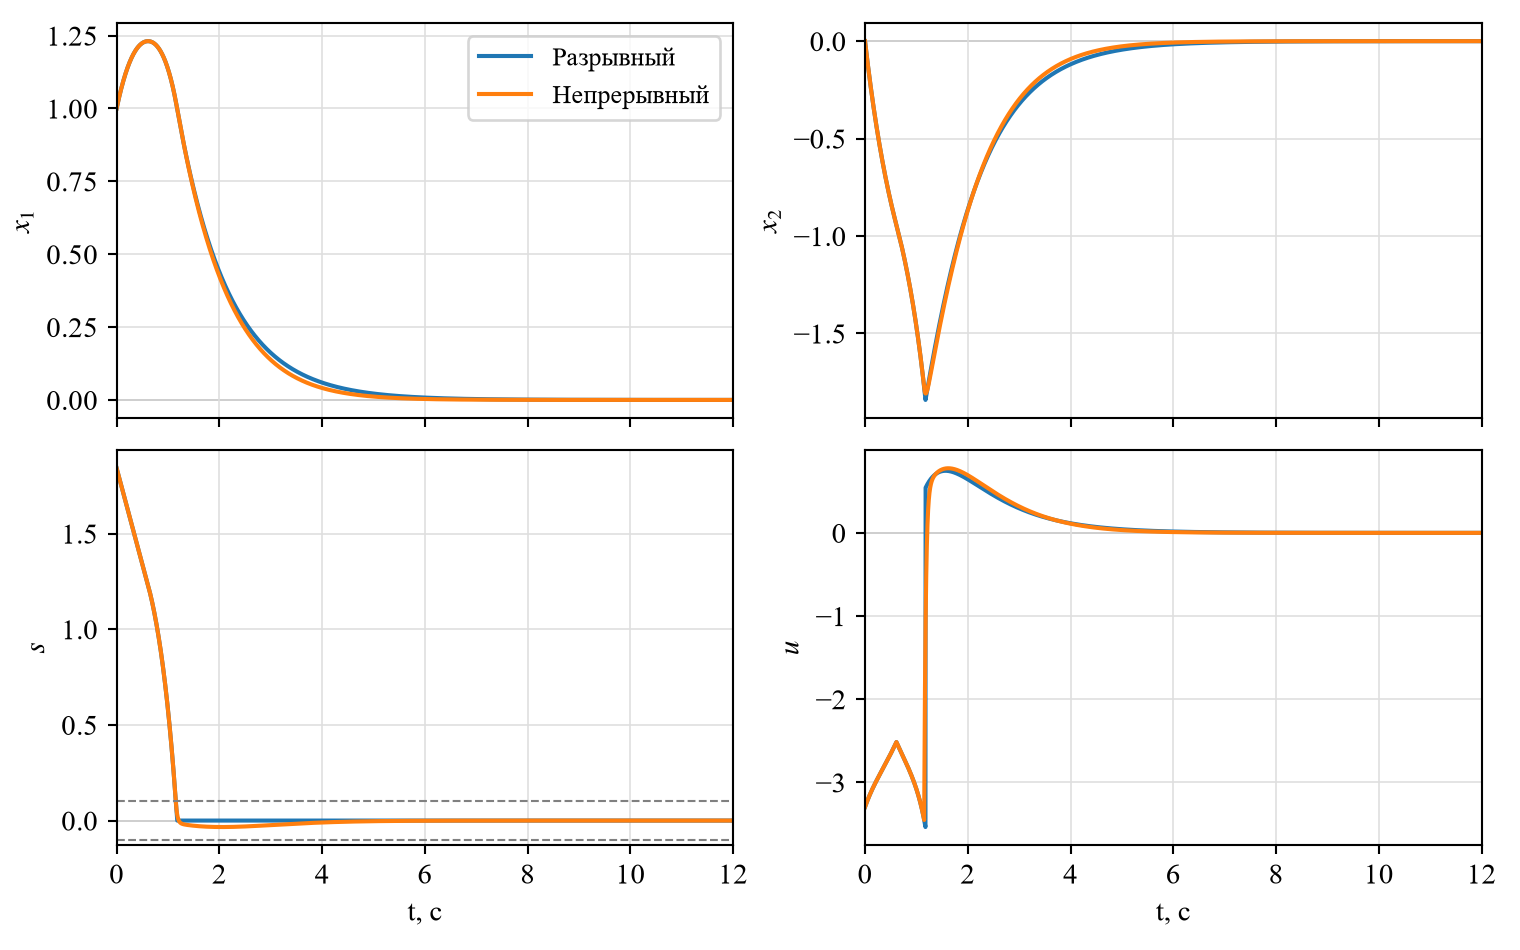
\includegraphics[width=0.95\textwidth]{../lab5/tex/images/task1_comparison.png}
 \caption{Первая система работы 5 Разрывный и непрерывный законы}
\end{guidefigure}

\subsection{Работа 5 Вторая система и робастный наклон поверхности}
\addition Для системы
\[
 \dot x_1=x_2+a_1x_1\sin x_1,\qquad
 \dot x_2=a_2x_1x_2+3u,\qquad a_1,a_2\in[0,2]
\]
параметр $a_1$ уже занят неизвестным коэффициентом объекта.
Поэтому наклон поверхности задаём непосредственно числом:
\[
 s=3x_1+x_2.
\]
На $s=0$ выполняется
\[
 \dot x_1=(-3+a_1\sin x_1)x_1,\qquad
 x_1\dot x_1\le-(3-2)x_1^2=-x_1^2.
\]
Число $3$ выбрано больше верхней границы $a_1$. Например,
наивная поверхность $s=x_1+x_2=0$ при $a_1=2$ допускает ненулевое
равновесие $x_1=\pi/6$, поскольку $-1+2\sin(\pi/6)=0$.
Она не обеспечивает требуемое глобальное притяжение к нулю.

Для выбранной поверхности
\[
 \dot s=3x_2+3a_1x_1\sin x_1+a_2x_1x_2+3u.
\]
Нормируем неопределённость на известный входной коэффициент $3$:
\[
 \left|x_2+a_1x_1\sin x_1+\frac{a_2}{3}x_1x_2\right|
 \le|x_2|+2|x_1\sin x_1|+\frac23|x_1x_2|=\varrho(x).
\]
Отсюда закон и его оценка:
\[
 \beta=\varrho+1,\qquad u=-\beta\sgn s,\qquad
 V=\frac{s^2}{2},\quad \dot V\le-3|s|,\quad
 t_*\le\frac{|s(0)|}{3}.
\]
До достижения $\frac{d}{dt}|x_1|\le-|x_1|+|s|$ почти всюду,
что даёт ограниченность. После достижения
\[
 |x_1(t)|\le|x_1(t_*)|e^{-(t-t_*)},\qquad x_2=-3x_1.
\]
Начало глобально асимптотически устойчиво для всех допустимых параметров.
Эквивалентный вход для отображения идеального скольжения равен
\[
 u_{eq}=3x_1-a_1x_1\sin x_1+a_2x_1^2.
\]
Последнее слагаемое положительно: оно получается из
$-a_2x_1x_2/3$ при $x_2=-3x_1$.
При $a_1=a_2=2$, $x(0)=(1{,}5;0)^T$ моделирование даёт
$t_*\approx0{,}163$ с, затем оба состояния сходятся к нулю.

\subsection{Работа 5 Непрерывное управление маятником}
\addition Задано уравнение
\[
 ml\ddot\theta+mg\sin\theta+kl\dot\theta
 =\frac{T}{l}+mh(t)\cos\theta,
\]
\[
 l\in[0{,}8;1],\quad m\in[0{,}5;1],\quad
 k\in[0{,}1;0{,}2],\quad |h(t)|\le0{,}5,\quad g=9{,}81.
\]
В этой задаче $g$ --- ускорение свободного падения, $h(t)$ --- внешнее
ускорение, $T$ --- управляющий момент. Это физические обозначения задания,
а не функции $g(x),h(x)$ из общего шаблона~\eqref{eq:sm-general}.
После деления на $ml$ имеем
\[
 \ddot\theta=-\frac gl\sin\theta-\frac km\dot\theta
             +\frac{T}{ml^2}+\frac{h(t)}l\cos\theta.
\]
Положим $x_1=\theta$, $x_2=\dot\theta$, $s=x_1+x_2$.
Умножая $\dot s$ на $ml^2$, получаем
\[
 ml^2\dot s=l^2(m-k)x_2-mgl\sin x_1+mlh(t)\cos x_1+T.
\]
Границы параметров дают $|l^2(m-k)|\le0{,}9$, $mgl\le9{,}81$,
$ml|h|\le0{,}5$. Поэтому подходит
\begin{equation}
 \varrho(x)=0{,}9|x_2|+9{,}81|\sin x_1|+0{,}5|\cos x_1|,
 \qquad T=-(\varrho+1)\sat(s/\varepsilon).
 \label{eq:pendulum-sat}
\end{equation}
Закон использует только угол, скорость и известные границы. Значения
$m,l,k$ и $h(t)$ ему не требуются.
При $|s|\ge\varepsilon$ для $V=s^2/2$ выполняется
\[
 \dot V\le-\frac{|s|}{ml^2}\le-|s|,
 \qquad t_\varepsilon\le\max\{|s(0)|-\varepsilon,0\},
\]
поскольку $ml^2\le1$. Полоса инвариантна. Для
$\tau=t-t_\varepsilon\ge0$ из $\dot\theta=-\theta+s$ следует
\[
 |\theta(t)|\le e^{-\tau}|\theta(t_\varepsilon)|
 +\varepsilon(1-e^{-\tau}),
\]
\[
 \limsup_{t\to\infty}|\theta(t)|\le\varepsilon,\qquad
 \limsup_{t\to\infty}|\dot\theta(t)|\le2\varepsilon.
\]
До входа $s$ ограничен, следовательно, угол и скорость также ограничены.
Гарантия глобальна по начальным условиям. При $\varepsilon=0{,}05$
предельные оценки составляют $0{,}05$ рад и $0{,}1$ рад/с.
Угол не обязан сразу после достижения полосы попасть в интервал
$[-\varepsilon,\varepsilon]$: в оценке ещё присутствует затухающая
зависимость от начального угла.

\subsubsection{Почему здесь гарантируется окрестность}

В состоянии $\theta=\dot\theta=0$ уравнение равновесия требует
\[
 T(0,0)=-mlh(t).
\]
Один непрерывный статический закон $T=T(\theta,\dot\theta)$ не может иметь
в нуле разные значения для всех неизвестных $h(t)$. При насыщении
в~\eqref{eq:pendulum-sat} $T(0,0)=0$, поэтому ненулевое ускорение
может вывести маятник из точного нуля. Для этой задачи корректно заявлять
глобальную \emph{практическую} стабилизацию, то есть достижение малой
заданной окрестности. Это принципиально отличается от первой системы,
в которой неопределённые слагаемые исчезают в нуле и точная сходимость
доказана отдельно.
